\documentclass[12pt]{article}

\usepackage{hyperref, tabularx, booktabs, amssymb,amsmath,amsfonts,eurosym,geometry,ulem,graphicx,caption,color,setspace,sectsty,comment,footmisc,caption,natbib,pdflscape,subfigure,array,hyperref, float, rotating}


\hypersetup{
    colorlinks=true,
    linkcolor=blue,
    filecolor=magenta,      
    urlcolor=cyan,
    pdftitle={Overleaf Example},
    pdfpagemode=FullScreen,
    }

\normalem

\onehalfspacing



\newcolumntype{L}[1]{>{\raggedright\let\newline\\arraybackslash\hspace{0pt}}m{#1}}
\newcolumntype{C}[1]{>{\centering\let\newline\\arraybackslash\hspace{0pt}}m{#1}}
\newcolumntype{R}[1]{>{\raggedleft\let\newline\\arraybackslash\hspace{0pt}}m{#1}}

\geometry{left=1.0in,right=1.0in,top=1.0in,bottom=1.0in}

\begin{document}

\begin{titlepage}
\title{Eviction, Education, and Identification Under Selection: Evidence from Ohio}
\author{Arjun Shanmugam}
\date{\today}
\maketitle
\begin{abstract}
\noindent I attempt to identify the causal effect of changes in the eviction rate on students' math and reading proficiency rates at the city level. Using data from Ohio and a fixed effects model, I estimate that a 1 percent increase in a city's eviction rate leads to a 0.064 percent decrease in its math proficiency rate. I find negative but insignificant effects on reading proficiency. In racially diverse cities, estimates are larger in magnitude and more significant. My fixed effects model controls for unobserved confounders that vary solely across cities or solely across time. But if unobserved confounders vary across both of these dimensions—which is likely—then my estimates are biased and the true causal effect is lower in magnitude than my findings suggest. I evaluate the plausibility of this concern by discussing eviction and its correlates and with an analysis of coefficient and $R^2$ stability when controls are introduced.\\

\bigskip
\end{abstract}
\setcounter{page}{0}
\thispagestyle{empty}
\end{titlepage}
\pagebreak \newpage




\doublespacing


\section{Introduction} \label{sec:introduction}
Fueled by stagnating incomes and rising housing costs, an eviction crisis has burdened low-income families in the United States for decades. It is estimated that over half of poor renting families spends over half its income on rent, meaning that unanticipated shocks can force families into homelessness \citep{desmond_evicted:_2017}. At various points beginning in March 2020, the federal government, the Centers for Disease Control, and some state and local governments implemented eviction moratoria, preventing a wave of evictions as pandemic-related lockdowns spread\citep{thrush_federal_2021, goldstein_landlords_2020}. But today, as moratoria expire, eviction rates are creeping up in cities across the country\citep{zaveri_after_2022}. A large body of research has investigated the effect of eviction on adults, but comparatively little evidence exists on how it affects children. If eviction impacts academic performance, then lifetime outcomes could be at stake.

This paper attempts to identify the causal effect of eviction on math and reading proficiency among third through eighth grade students. Ideally, longitudinal microdata would allow me to compare the test scores of children who have experienced eviction with the test scores of those who have not. Lacking this data, I am faced with the choice of conducting my analysis at the school district level or the city level. If eviction reduces test scores, and evicted students tend to move to different districts upon eviction, then an analysis at the school district level might underestimate the true effect of eviction. If students tend to attend school within the same \textit{city} upon being evicted, any change in their academic performance should be visible in city level data. Thus, I aggregate education and eviction data to the city level.

I draw the majority of my data from two sources. The first is The Eviction Lab at Princeton University, which has compiled a database of evicton rates over the 2000s and 2010s in nearly every city in the United States\citep{desmond_eviction_2018}. These data come from formal eviction records held by a number of public and private sector sources. The Eviction Lab also provides ACS 5-year estimates of time-varying socioeconomic characteristics of many of the cities in which it tracks eviction rates, such as the poverty rate and the percent homes which are renter occupied. My second source of data is the Ohio Department of Education, which provides district-level data on the portion of students judged proficient in math and reading from the 2005-06 school year to the 2014-2015 school year. In order to expand my set of controls, I also obtain ACS 5-year estimates of educational attainment at the city level. I build a novel panel dataset of eviction rates, math and reading proficiency scores, and a host of time-varying socioeconomic characteristics at the city-year level.

My biggest econometric challenge is that the treatment I seek to evaluate—eviction—is nonrandom. Partly due to generations of housing policies which sought to systematically exclude African-Americans from home ownership, eviction is strongly correlated with race \citep{rothstein_color_2017}. Eviction is also correlated with income, renter-occupied rates, and a host of other socioeconomic variables, many of which are also correlated with test scores. I address the threat to identification posed by observable confounders with a comprehensive set of controls.

Still, without a random source of variation in eviction rates, it is likely that eviction rates are correlated with unobserved characteristics of cities \footnote{Using \cite{kroeger_nuisance_2020}'s result that nuisance ordinances increase eviction rates, I attempted to instrument eviction rates using the presence of a nuisance ordinance in a city-year. Ultimately, the first-stage was too weak to produce precise instrumental variable estimates; I continue in search of an exogenous source of variation.}. Using year and city fixed effects, I am able to control for unobserved, city-specific characteristics which are constant over time and unobserved, year-specific characteristics which are constant across cities. But time-variant unobservables—say, changes in landlords' attitudes towards tenants within a single city over time—may still bias my estimates. I do not claim to overcome this threat to identification. However, in Section 5, I argue that observed characteristics explain most of the variation in eviction rates and bound the bias in my estimated coefficients following \cite{oster_unobservable_2019}.

I contribute to a wide literature which studies the effects of eviction on important determinants of well being. Evicted mothers are more likely to be depressed; low-income workers are more likely to lose their jobs after being evicted; and at the height of the pandemic, eviction moratoria limited households’ food insecurity and mental stress\citep{desmond_housing_2016, desmond_evictions_2015, an_covid-19_2021}. Less research has focused on the effects of evictions on children. \cite{grigg_school_2012} finds that residence changes negatively affect outcomes such as academic achievement and social development, but evictions are traumatic for children in ways that voluntary moves are not. For this reason, and because education is central to the development of children, I hope to estimate the causal effect of eviction on test scores.

Section 2 discusses in greater depth the data I obtain and the dataset I assemble for my analysis. Section 3 outlines my empirical strategy. Section 4 provides and discusses results, and Section 6 concludes.
















\section{Background and Data} \label{sec:data}
The data used in this analysis come from three sources. I limit my analysis to the state of Ohio for two reasons. First, variation in eviction policy is relatively small across cities in Ohio (\textbf{CITE}). This makes it more plausible that variation in eviction rates is random and not correlated with policy-related unobservables which might also affect academic performance. Second, by omitting other states from the analysis, I avoid the possibility that time and state-varying confounders—which state fixed effects cannot control for—bias my estimates.
\subsection{Eviction Data}
Eviction cases in America are usually tried in civil courts at the county-level. Most cases are resolved in one of three ways. An \textit{eviction judgement} can be rendered, "ordering the defendants to vacate a premise by a specific date"; the case can be \textit{dismissed}, "or ruled in favor of the defendant"; or the judge can permit a \textit{mediated agreement} between the landlord and the tenant, establishing certain terms of payment and resulting in an eviction judgement if these terms are unmet\citep{desmond_eviction_2018}. In all three cases, courts generally keep records of evictions that include information such as landlord and tenant names and addresses, case rulings, and the date the case was heard.

I obtain eviction data from The Eviction Lab, which has collected millions of the above described records in two ways: first, by sending requests to state and county governments, and second, by purchasing records from two private companies. State and county records are publicly accessible under the Freedom of Information Act; about 12 million records were obtained in this manner. LexisNexis Risk Solutions and American Information Research Services, Inc. provided approximately 67 million and 11 million eviction records respectively. The Eviction Lab geocoded tenant addresses so that they could be linked to U.S. Census-designated cities, then aggregated records to the city-level to protect privacy and calculate eviction rates for each city during almost every year in the 2000s and 2010s. The Eviction Lab also merged socioeconomic variables taken from the American Community Survey's (ACS) 2010 and 2015 five-year estimates: racial composition variables, the percent of households which are renter occupied, poverty rate, median household income, and median property value.

\subsection{Testing Data}
I obtain educational testing data from the Ohio Department of Education. The Ohio Department of Education implemented its current testing regime, the Ohio Achievement Assessment (OAA), soon after the passage of the No Child Left Behind Act, which required states to assess third through eighth grade students in reading and math \citep{fox_examination_2014}. I note that in  2010, the educational benchmarks used by the OAA were updated to incorporate the Common Core State Standards—a set of academic standards meant to ensure that all state curricula reached the same level of rigor \citep{ohio_school_boards_association_ohios_2010}. Year fixed effects should control for these changes in the way the OAA defined proficiency.

The Ohio Department of Education has made OAA proficiency rates in math and reading at the school district-grade level available since the 2005-06 school year. I assemble this data into a single, school district-school year level dataset. Assessments are given in the spring, so I denote each school year by the year of its spring term (i.e., test scores from the 2005-06 school year are coded as coming from the year 2006). Using the National Center for Education Statistics (NCES) geographic relationship files, I match each school district to the city or cities that it intersects with. When a school district spans two cities, I calculate its \textit{adjusted enrollment} by dividing its total enrollment in each year equally across the cities it spans. Then, I aggregate the data to the city-year level. I calculate each city-year's proficiency rate in each subject as the mean of proficiency rates in the school districts spanned by the city, weighted by adjusted enrollment.

I then merge each city-year from the eviction data with the following city-year from the education data. The OAA is generally administered in May of each year. If I were to match on identical city-years, I would risk attempting to draw a causal link between evictions and performance on a standardized test which occurred in the past.


\subsection{Descriptive Statistics}
Table 1 presents descriptive statistics for the sample. Math and reading proficiency rates are about 77 and 83 percent respectively. There is significant variation in both math and proficiency rates as well, with standard deviations of around 13 percent for math and 10 percent for reading.

Important for the precision of my estimates is the fact that there is also a great deal of variation in eviction rates. The standard deviation of eviction rates is about equal to the mean eviction rate in the data. The wide range of  eviction rates—in the city-year with the highest eviction rate, nearly 27 percent of households were evicted—paints a picture of vast inequality in housing security across Ohioan cities.

I also present summary statistics for control variables which I include in my regression model. I discuss later why these controls are important and correlated with both the dependent and independent variables.



\section{Empirical Strategy} \label{sec:empirical_strategy}
I first provide correlational evidence of the relationship between eviction and math and reading proficiency rates in Figure 1. Figure 1's plots were generated using the binscatter package in Stata \citep{stepner_binscatter:_2013}. To construct these figures, city-years were sorted by eviction rate and separated into 20 equal sized bins. Then, the mean math and reading proficiency rate was calculated for each bin. Each bin was plotted according to its mean eviction rate on the x-axis and its mean math and reading proficiency rate on the y-axis. Lastly, an OLS-estimated line of best fit was plotted on top of each graph. While these figures do not display causal relationships, they provide evidence of strikingly lower proficiency rates in high eviction areas.  Specifically, a one percent increase in a city-year's eviction rate is associated with a \textbf{FILL} percent decrease in its math proficiency rate and a \textbf{FILL} percent decrease in its reading proficiency rate.

The OLS coefficients estimated to create Figure 1's lines of best fit are biased by observed confounders. Figure 2 displays heatmaps of census-designated cities in Cuyahoga County—the county containing Cleveland. Each heatmap visualizes the values of one variable over the cities of Cuyahoga County. I chose to create heatmaps for the dependent variables, the independent variable of interest, and a select number controls. To create each heatmap, I first calculate the mean value of a single variable over the sample period for each city. Then, I sort each city by its calculated mean. Lastly, I bin cities into four equally sized bins and color each city on the map according to the bin it falls into. Poverty rates and renter occupied rates are positively correlated with eviction rates and negatively correlated with math and reading proficiency. Median household income is negatively correlated with eviction rate and positively correlated with math and reading proficiency rates. My empirical model must control for these observed confounders and others.

It is also possible that there are unobserved differences across cities which bias my estimates. For instance, time-invariant cultural differences across cities might affect both proficiency rates and eviction rates. Shocks that affect all cities within a certain year–say, hardship resulting from the Global Financial Crisis, which occurs during the period I study—might also bias my estimates. To control for these phenomena, I must add year and city fixed effects to my model.

I estimate the impact of a one percent change in the eviction rate on outcome variables using the following models
\begin{equation}
m_{itg} = \beta_{math} E_{it} + \delta_i + \gamma_t + \phi_g + \chi_{it} + \epsilon_{itg}
\end{equation}
\begin{equation}
r_{itg} = \beta_{read} E_{it} + \delta_i + \gamma_t + \phi_g + \chi_{it} + \epsilon_{itg}
\end{equation}
where $m_{itg}$ is the math proficiency rate in city $i$ in year $t$ and grade $g$, $r_{itg}$ is the reading proficiency rate in city $i$ in year $t$ and grade $g$, $E_{it}$ is the eviction rate in  city $i$ during year $t$, $\delta_i$ is a city fixed effect, $\gamma_t$ is a year fixed effect, $\phi_g$ is a grade fixed effect, $\chi_{it}$ represents city-specific, time-varying controls, and $\epsilon_{itg}$ is an error term. I note that $\beta_{math}$ and $\beta_{read}$ are my coefficients of interest.


\section{Results and Discussion} \label{sec:result}
\subsection{Main Results}
In Table 2, I estimate equations (1) and (2) on my entire sample. Columns (1)-(4) show that after the addition of city and year fixed effects, estimates of $\beta_{math}$ are relatively stable. Column (4) includes city, year, and grade fixed effects along with socioeconomic controls, and is thus my preferred estimate. According to my results, a one percent increase in a city-year's eviction rate is associated with a 0.064 percent decrease in its math proficiency rate. The magnitude of the coefficient is just over two times the standard error; about 66 percent of the variation in math proficiency rates is explained by the independent variables. These results suggest that within cities, even conditional on a set of socioeconomic controls, higher eviction rates are associated with lower mathematics proficiency rates. Columns (5)-(8) show estimates of $\beta_{read}$. While these estimates are also relatively stable, they are largely insignificant. Here, column (8) is my preferred estimate.
    
One possible explanation for the fact that estimates of $\beta_{read}$ are less significant than estimates of $\beta_{math}$ is that children's reading performance depends more on their home environments than math performance. Indeed, this explanation is consistent with the literature, which agrees that "word-reading accuracy and fluency ... is linked to aspects of the family environment that children grow up in" \citep{van_bergen_why_2017}.

\subsection{Heterogeneous Treatment Effects}
Next, I investigate the possibility that the association between eviction rates and proficiency rates may be different for particular subsets of the sample. I calculate a median for each control variable besides grade year and year. Then, I estimate equations (1) and (2) separately on observations above the median and below the median. 

Figure 3 presents the values of $\beta_{math}$ from these regressions. Each point represents the estimate of $\beta_{math}$ in a single regressions. Labels on the y-axis indicate the sample on which equation (1) was estimated. Blue points correspond to estimates on below-median samples, while red points correspond to above-median samples. The key insight of Figure 3 is that in general, $\beta_{math}$ is more negative and more significant in more diverse and socioeconomically distressed areas. Consider the coefficients corresponding to the "High pct. white sample" and the "Low pct. white sample". When estimated on the "Low pct. white sample," $\beta_{math}$ is lower and more significant. One interpretation of these differences is that in more diverse and socioeconomically distressed cities, evicted students have access to weaker support systems, meaning that their academic performance suffers more after a forced move. 

Figure 4 presents heterogeneous treatment effects on reading proficiency rates analogously to Figure 3. In keeping with main results presented in Table 2, the estimated values of $\beta_{read}$ are smaller in magnitude and insignificant than estimated values of $\beta_{math}$. One would expect treatment effects on reading proficiency to be more negative in socioeconomically distressed cities; perhaps children in these cities do not have access to the same at-home environments as children in wealthier areas. However, this hypothesis is not supported by Figure 3 as there is no distinguishable trend when socioeconomically distressed areas are compared to non-socioeconomically distressed areas.

\subsection{Validity of Estimates As Causal}
Without exogenous variation in eviction rates, the validity of my estimates as causal is still in question. I begin by discussing the shortcomings of the controls I include. While these controls explain a large portion of the variation in math and reading proficiency rates, the most obvious shortcoming of my identification strategy is the lack of educational attainment rates as controls. Educated individuals are more likely to be wealthy, making them less likely to be evicted. Educated individuals are also more likely to have the time and resources to navigate the eviction process when faced with eviction filings. And plenty of research shows that parental education is correlated with children's educational outcomes \citep{havemen}. Unfortunately, ACS 5-year estimates are not available for the portion of adults with bachelor's degrees in a large portion of the cities in my sample. Because educational attainment is negatively correlated with eviction and positively correlated with child educational performance, this omission in theory biases my estimates negatively. 


Time-varying confounders pose a still greater threat to my identification strategy. For instance, under the No Child Left Behind Act, low-performing Ohio schools were required to offer free tutoring to parents if they missed "adequate yearly progress" standards set by the Ohio Department of Education \citep{klein_no_2015}. Consider the case of a school which meets this standard during parts of the sample period and does not during others. If such schools exist in my sample, they could confound my estimates of $\beta_{math}$ and $\beta_{read}$.


To assess the extent to which these confounders might bias my estimates, I take two approaches. In the first, I regress \emph{pct. proficient in math}, \emph{pct. proficient in reading}, and \emph{eviction rate} separately on my controls. I estimate each regression using four sets of controls and analyze how $R^2$ values change as more controls are added. The results of this analysis are presented in Table 3.

\textbf{TRY OSTER APPROACH}


My exploration of heterogeneous treatment effects in subsection 4.2 suggests another possibility: that treatment effects are balancing each other out within cities, pushing my estimates towards zero. Because I do not have access to individual-level data, I am forced to rely on city-year averages in my analysis. For an instructive example as to how this might alter my results, consider the city of Akron. Overall, Akron is relatively poor; it ranks in the top 30 of Ohio's highest-poverty cities and its mean eviction rate over the sample period is among the highest of the cities I observe. Akron intersects seven different school districts, including Revere Local School District and Akron Public Schools District. In Revere Local School District, 91.6 percent of students have access to broadband internet and median household income is \$109,173 (NCES District Demographic Dashboard). In Akron Public Schools District, just 77.1 percent do; the median household makes \$38,006 each year. Evicted students in districts such as Revere Local may have access to support systems which allow them to fare better academically than students attending Akron Public Schools. This suggests that the true effect of eviction on proficiency is more negative for an Akron Public Schools student than a Revere Local student. In fact, it is plausible that the true effect of eviction on proficiency for the average Revere Local Schools student is indistinguishable from zero. 

If I had perfect data on the number of students from each school district which reside in each city in each year—and could thus construct a \textit{precise} weighted average of district test scores for each city-year—then this phenomenon would not bias my estimates. But I do not have such data, and so when a district intersects with two or more cities, I am forced to assume that its student body resides evenly across those cities. Revere Local Schools, for example, intersects five cities. If the true portion of Revere Local Schools' students residing in Akron is less than one-fifth, then I am over-weighting the treatment effect in Revere Local Schools' in my calculation of the treatment effect for the city of Akron. If this over-weighting of wealthy school districts' test scores in the calculation of city-year level test scores for poor, high-eviction cities happens systematically in my analysis, then my obtained coefficients are biased upwards.


\section{Conclusion} \label{sec:conclusion}



\singlespacing
\setlength\bibsep{0pt}
\bibliographystyle{rusnat}
\bibliography{citations}



\clearpage

\onehalfspacing


\begin{landscape}
\section*{Tables} \label{sec:tab}
\addcontentsline{toc}{section}{Tables}
\begin{table}[htbp]\centering
\def\sym#1{\ifmmode^{#1}\else\(^{#1}\)\fi}
\caption{Descriptive Statistics}
\begin{tabular}{l*{1}{ccccc}}
\toprule
                    &        Mean&          SD&         Min&         Max&           N\\
\midrule
\emph{Dependent variables}&            &            &            &            &            \\
\hspace{0.25cm} Pct. proficient in math&       77.25&       12.53&        1.50&      100.00&       66873\\
\hspace{0.25cm} Pct. proficient in reading&       82.82&        9.81&        8.30&      100.00&       66880\\
\vspace{0.1em} \\ \emph{Independent variable of interest}&            &            &            &            &            \\
\hspace{0.25cm} Eviction rate&        2.13&        2.14&        0.00&       26.83&       66882\\
\vspace{0.1em} \\ \emph{Control variables}&            &            &            &            &            \\
\hspace{0.25cm} Grade year&           6&           2&           3&           8&       66882\\
\hspace{0.25cm} Median household income&    49542.87&    21974.85&     2499.00&   250001.00&       65646\\
\hspace{0.25cm} Median property value&   119605.26&    76161.90&     9999.00&  1157600.00&       65862\\
\hspace{0.25cm} Pct. renter-occupied&       28.04&       14.23&        0.00&      100.00&       66882\\
\hspace{0.25cm} Pct. white&       91.06&       13.29&        0.00&      100.00&       66882\\
\hspace{0.25cm} Poverty rate&       10.78&        9.61&        0.00&      100.00&       66882\\
\hspace{0.25cm} Year&        2011&           3&        2006&        2015&       66882\\
\bottomrule
\multicolumn{6}{l}{\footnotesize Note: This table presents descriptive statistics for the sample. Descriptive statistics for \emph{Grade year} and \emph{Year} are }\\
\multicolumn{6}{l}{\footnotesize truncated to have zero decimal places. Values of independent and control variables are from the current year; values}\\
\multicolumn{6}{l}{\footnotesize of dependent variables are from the following year.}\\
\end{tabular}
\end{table}

\end{landscape}


\begin{table}[htbp]\centering
\def\sym#1{\ifmmode^{#1}\else\(^{#1}\)\fi}
\caption{Main Results}
\begin{tabular}{l*{8}{c}}
\toprule
                    &\multicolumn{4}{c}{Pct. Proficient in Math}        &\multicolumn{4}{c}{Pct. Proficient in Reading}     \\\cmidrule(lr){2-5}\cmidrule(lr){6-9}
                    &\multicolumn{1}{c}{(1)}&\multicolumn{1}{c}{(2)}&\multicolumn{1}{c}{(3)}&\multicolumn{1}{c}{(4)}&\multicolumn{1}{c}{(5)}&\multicolumn{1}{c}{(6)}&\multicolumn{1}{c}{(7)}&\multicolumn{1}{c}{(8)}\\
                    &        b/se&        b/se&        b/se&        b/se&        b/se&        b/se&        b/se&        b/se\\
\midrule
Eviction rate       &       0.016&      -0.065&      -0.065&      -0.062&       0.031&      -0.037&      -0.037&      -0.029\\
                    &      (0.04)&      (0.03)&      (0.03)&      (0.03)&      (0.03)&      (0.02)&      (0.02)&      (0.02)\\
\midrule
Observations        &       66873&       66873&       66873&       65073&       66880&       66880&       66880&       65080\\
Number of clusters  &        1189&        1189&        1189&        1184&        1189&        1189&        1189&        1184\\
$\text{R}^2$        &       0.459&       0.548&       0.659&       0.662&       0.474&       0.587&       0.660&       0.663\\
Place F.E.          &         Yes&         Yes&         Yes&         Yes&         Yes&         Yes&         Yes&         Yes\\
Year F.E.           &          No&         Yes&         Yes&         Yes&          No&         Yes&         Yes&         Yes\\
Grade F.E.          &          No&          No&         Yes&         Yes&          No&          No&         Yes&         Yes\\
Socioeconomic controls&          No&          No&          No&         Yes&          No&          No&          No&         Yes\\
\bottomrule
\multicolumn{9}{l}{\footnotesize Note: This table presents OLS regression estimates of the effect of \emph{eviction rate} on mathematics and reading}\\
\multicolumn{9}{l}{\footnotesize proficiency rates. Each column represents one regression. All regressions control for \emph{pct. white}, \emph{poverty rate},}\\
\multicolumn{9}{l}{\footnotesize \emph{pct. renter occupied}, \emph{median household income}, and \emph{median property value}. Robust standard errors}\\
\multicolumn{9}{l}{\footnotesize clustered at the city-level.}\\
\end{tabular}
\end{table}


\newpage
\begin{landscape}
\begin{table}[htbp]\centering
\def\sym#1{\ifmmode^{#1}\else\(^{#1}\)\fi}
\caption{Predictive Ability of Controls}
\begin{tabular}{l*{12}{c}}
\toprule
                    &\multicolumn{4}{c}{Pct. proficient in math}        &\multicolumn{4}{c}{Pct. proficient in reading}     &\multicolumn{4}{c}{Eviction rate}                  \\\cmidrule(lr){2-5}\cmidrule(lr){6-9}\cmidrule(lr){10-13}
                    &\multicolumn{1}{c}{(1)}&\multicolumn{1}{c}{(2)}&\multicolumn{1}{c}{(3)}&\multicolumn{1}{c}{(4)}&\multicolumn{1}{c}{(5)}&\multicolumn{1}{c}{(6)}&\multicolumn{1}{c}{(7)}&\multicolumn{1}{c}{(8)}&\multicolumn{1}{c}{(9)}&\multicolumn{1}{c}{(10)}&\multicolumn{1}{c}{(11)}&\multicolumn{1}{c}{(12)}\\
                    &        b/se&        b/se&        b/se&        b/se&        b/se&        b/se&        b/se&        b/se&        b/se&        b/se&        b/se&        b/se\\
\midrule
\hspace{0.25cm} Pct. white&            &            &            &     -11.992&            &            &            &      -5.299&            &            &            &       2.185\\
                    &            &            &            &         (.)&            &            &            &         (.)&            &            &            &         (.)\\
\hspace{0.25cm} Pct. renter-occupied&            &            &            &      -8.899&            &            &            &      -4.313&            &            &            &       1.295\\
                    &            &            &            &         (.)&            &            &            &         (.)&            &            &            &         (.)\\
\hspace{0.25cm} Poverty rate&            &            &            &       0.000&            &            &            &       0.000&            &            &            &       0.000\\
                    &            &            &            &         (.)&            &            &            &         (.)&            &            &            &         (.)\\
\hspace{0.25cm} Median household income&            &            &            &       0.000&            &            &            &       0.000&            &            &            &       0.000\\
                    &            &            &            &         (.)&            &            &            &         (.)&            &            &            &         (.)\\
\hspace{0.25cm} Median property value&            &            &            &       0.000&            &            &            &       0.000&            &            &            &       0.000\\
                    &            &            &            &         (.)&            &            &            &         (.)&            &            &            &         (.)\\
\midrule
$\mathbf{R^2}$      &\textbf{0.0}&\textbf{0.1}&\textbf{0.8}&\textbf{0.8}&\textbf{0.0}&\textbf{0.2}&\textbf{0.6}&\textbf{0.6}&\textbf{0.0}&\textbf{1.0}&\textbf{1.0}&\textbf{1.0}\\
Place F.E.          &         Yes&         Yes&         Yes&         Yes&         Yes&         Yes&         Yes&         Yes&         Yes&         Yes&         Yes&         Yes\\
Year F.E.           &          No&         Yes&         Yes&         Yes&          No&         Yes&         Yes&         Yes&          No&         Yes&         Yes&         Yes\\
Grade F.E.          &          No&          No&         Yes&         Yes&          No&          No&         Yes&         Yes&          No&          No&         Yes&         Yes\\
Socioeconomic controls&          No&          No&          No&         Yes&          No&          No&          No&         Yes&          No&          No&          No&         Yes\\
\bottomrule
\multicolumn{13}{l}{\footnotesize Note: This table presents OLS regression estimates of the effect of \emph{eviction rate} on mathematics and reading}\\
\multicolumn{13}{l}{\footnotesize proficiency rates. Each column represents one regression. All regressions control for \emph{pct. white}, \emph{poverty rate},}\\
\multicolumn{13}{l}{\footnotesize \emph{pct. renter occupied}, \emph{median household income}, and \emph{median property value}. Robust standard errors}\\
\multicolumn{13}{l}{\footnotesize are clustered at the city-level.}\\
\end{tabular}
\end{table}

\end{landscape}


\clearpage

\section*{Figures} \label{sec:fig}
\addcontentsline{toc}{section}{Figures}

\begin{figure}[H]
    \centering
    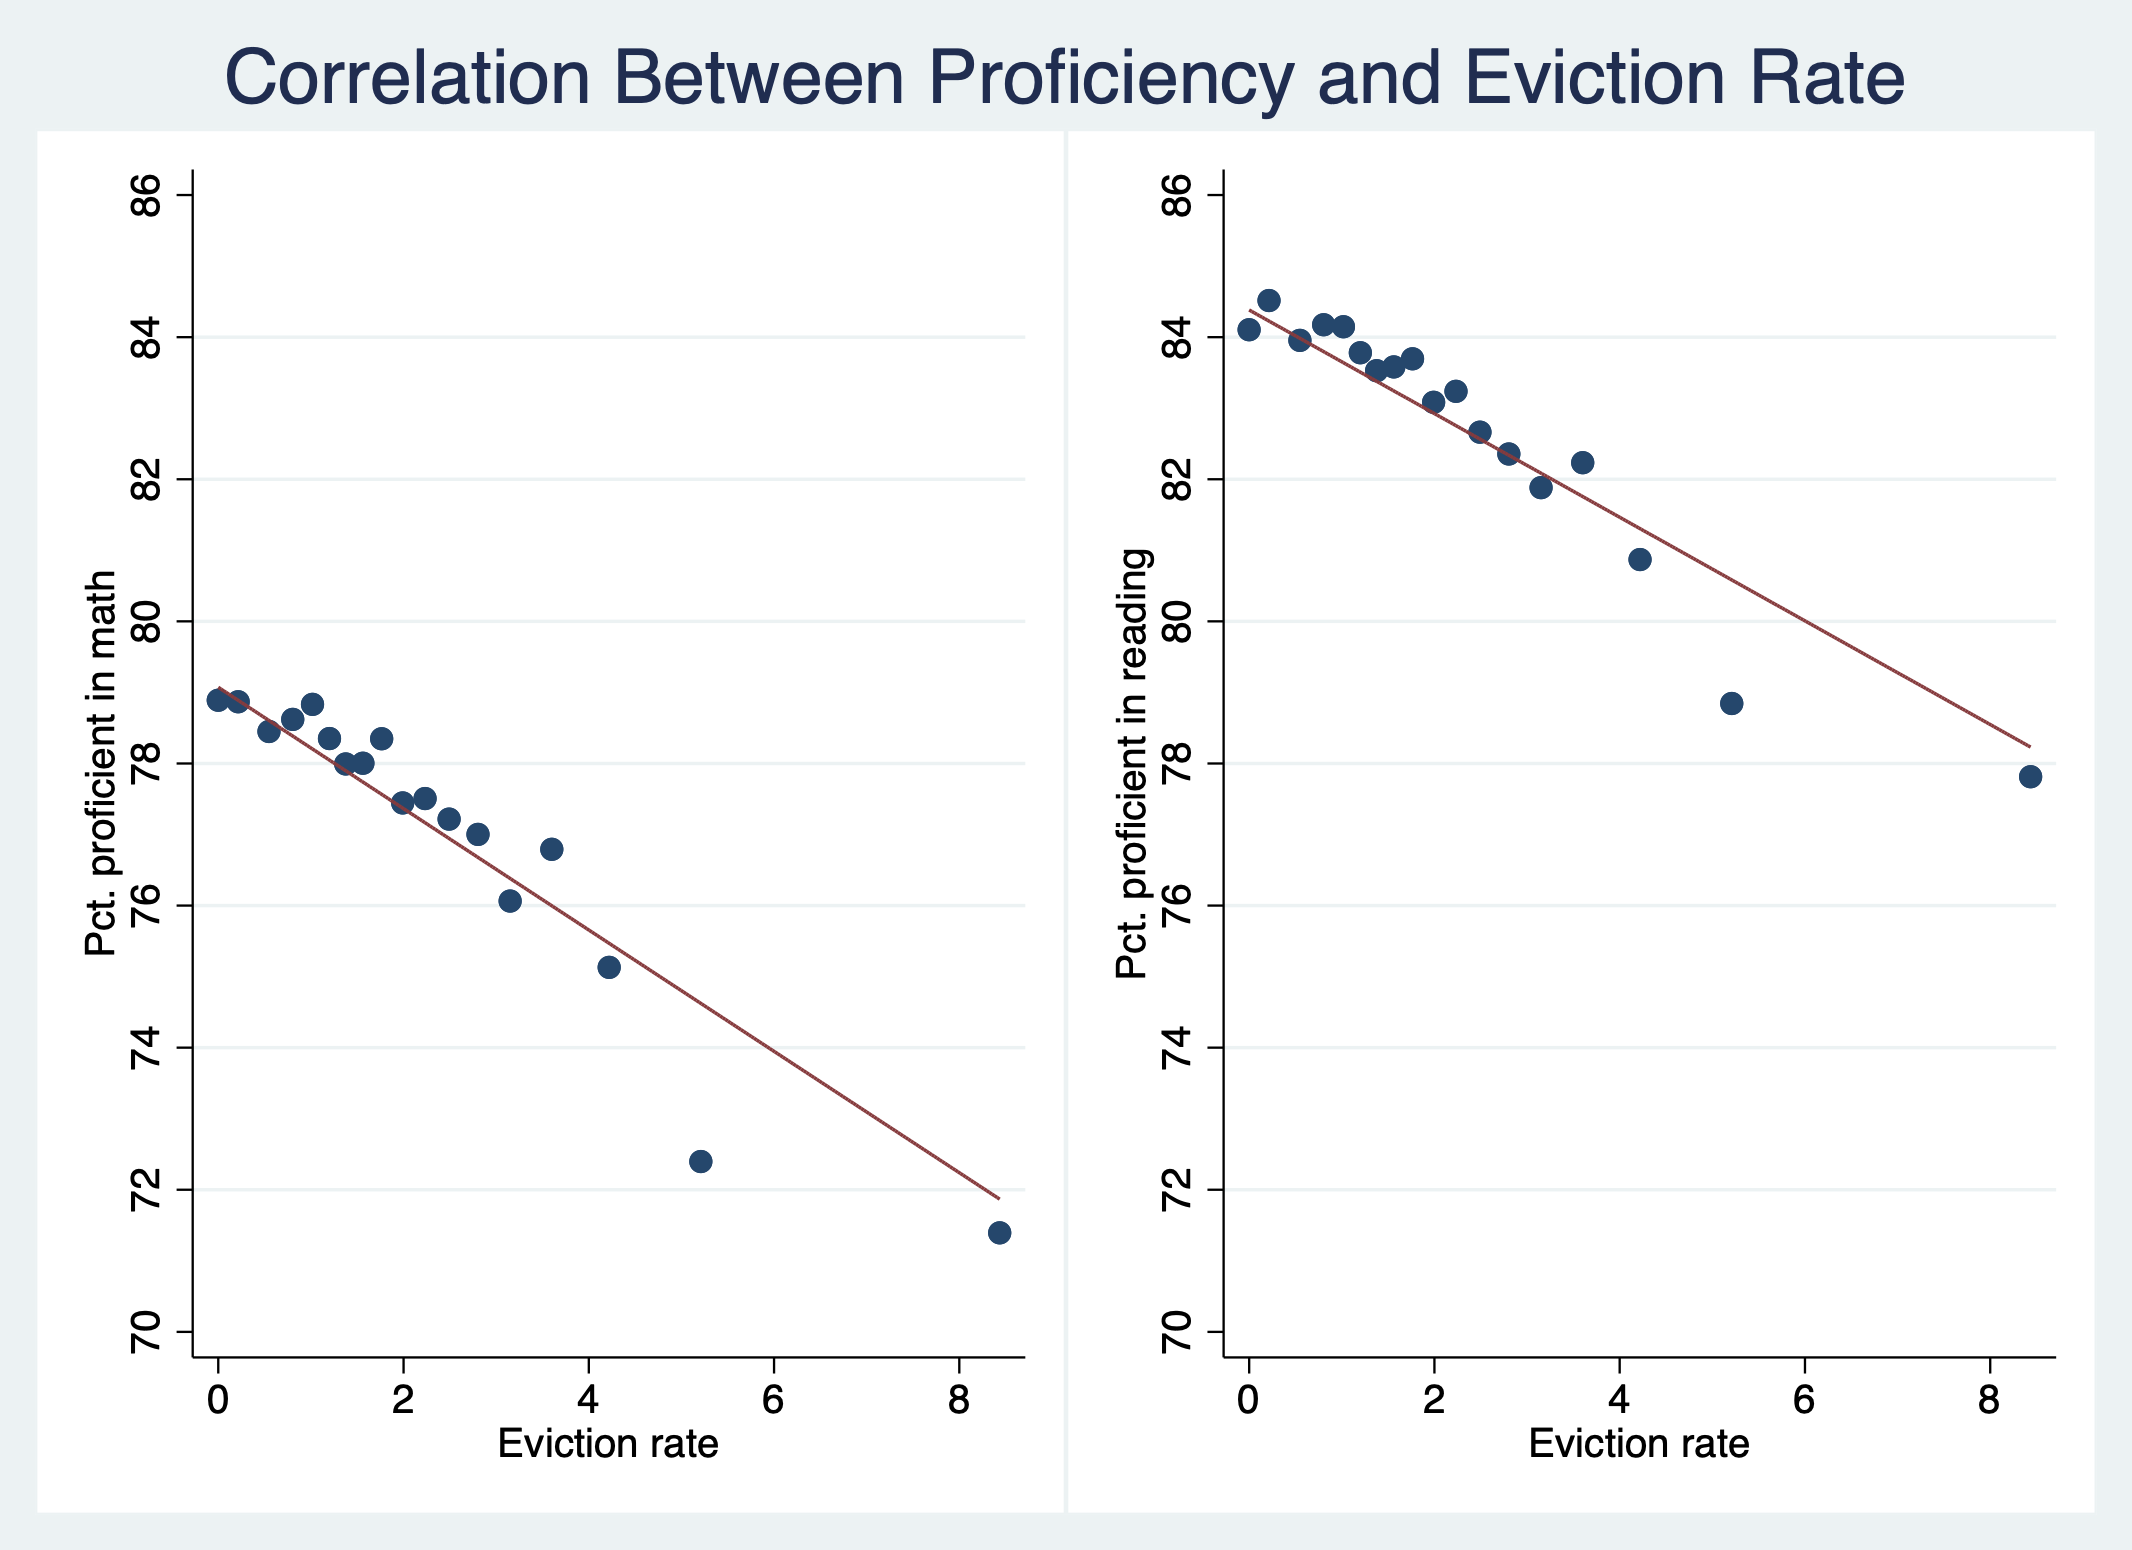
\includegraphics[scale=0.4]{output/graphs/outcome_binscatter.png}
    \caption{}
    \label{fig:my_label}
\end{figure}

\begin{landscape}
\begin{figure}
    \centering
    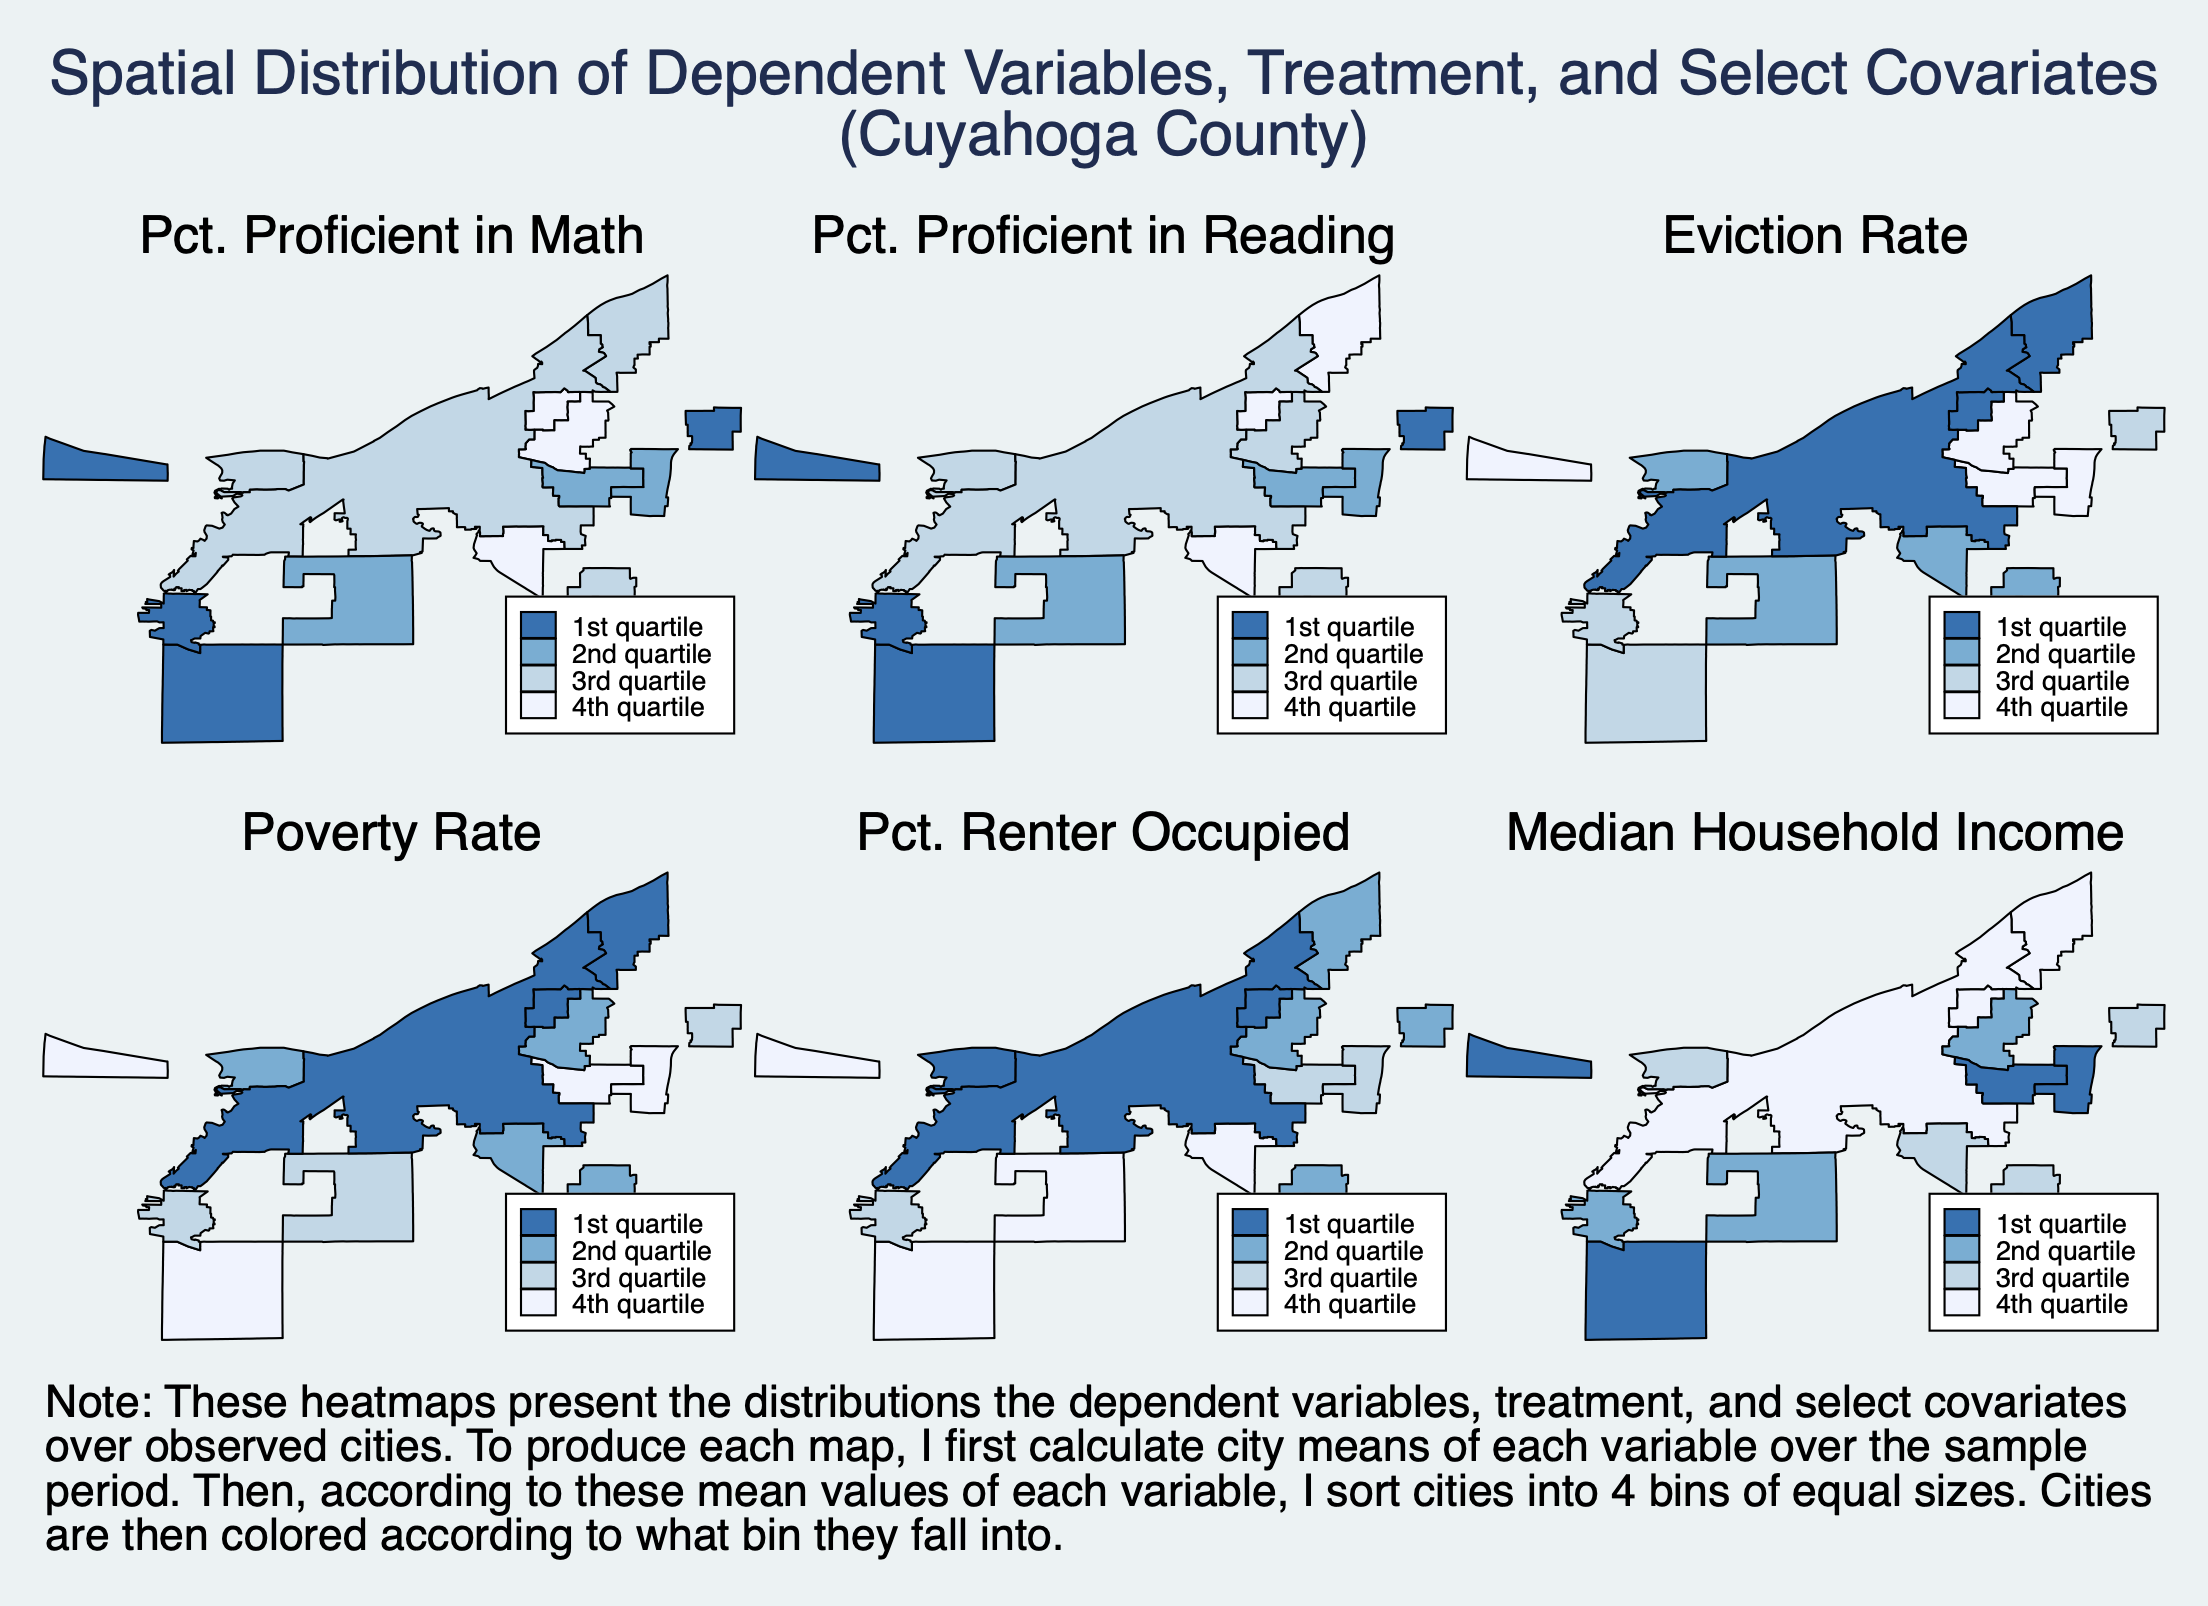
\includegraphics[scale=0.5]{output/graphs/maps.png}
    \caption{}
    \label{fig:my_label}
\end{figure}
\end{landscape}

\begin{landscape}
\begin{figure}
    \centering
    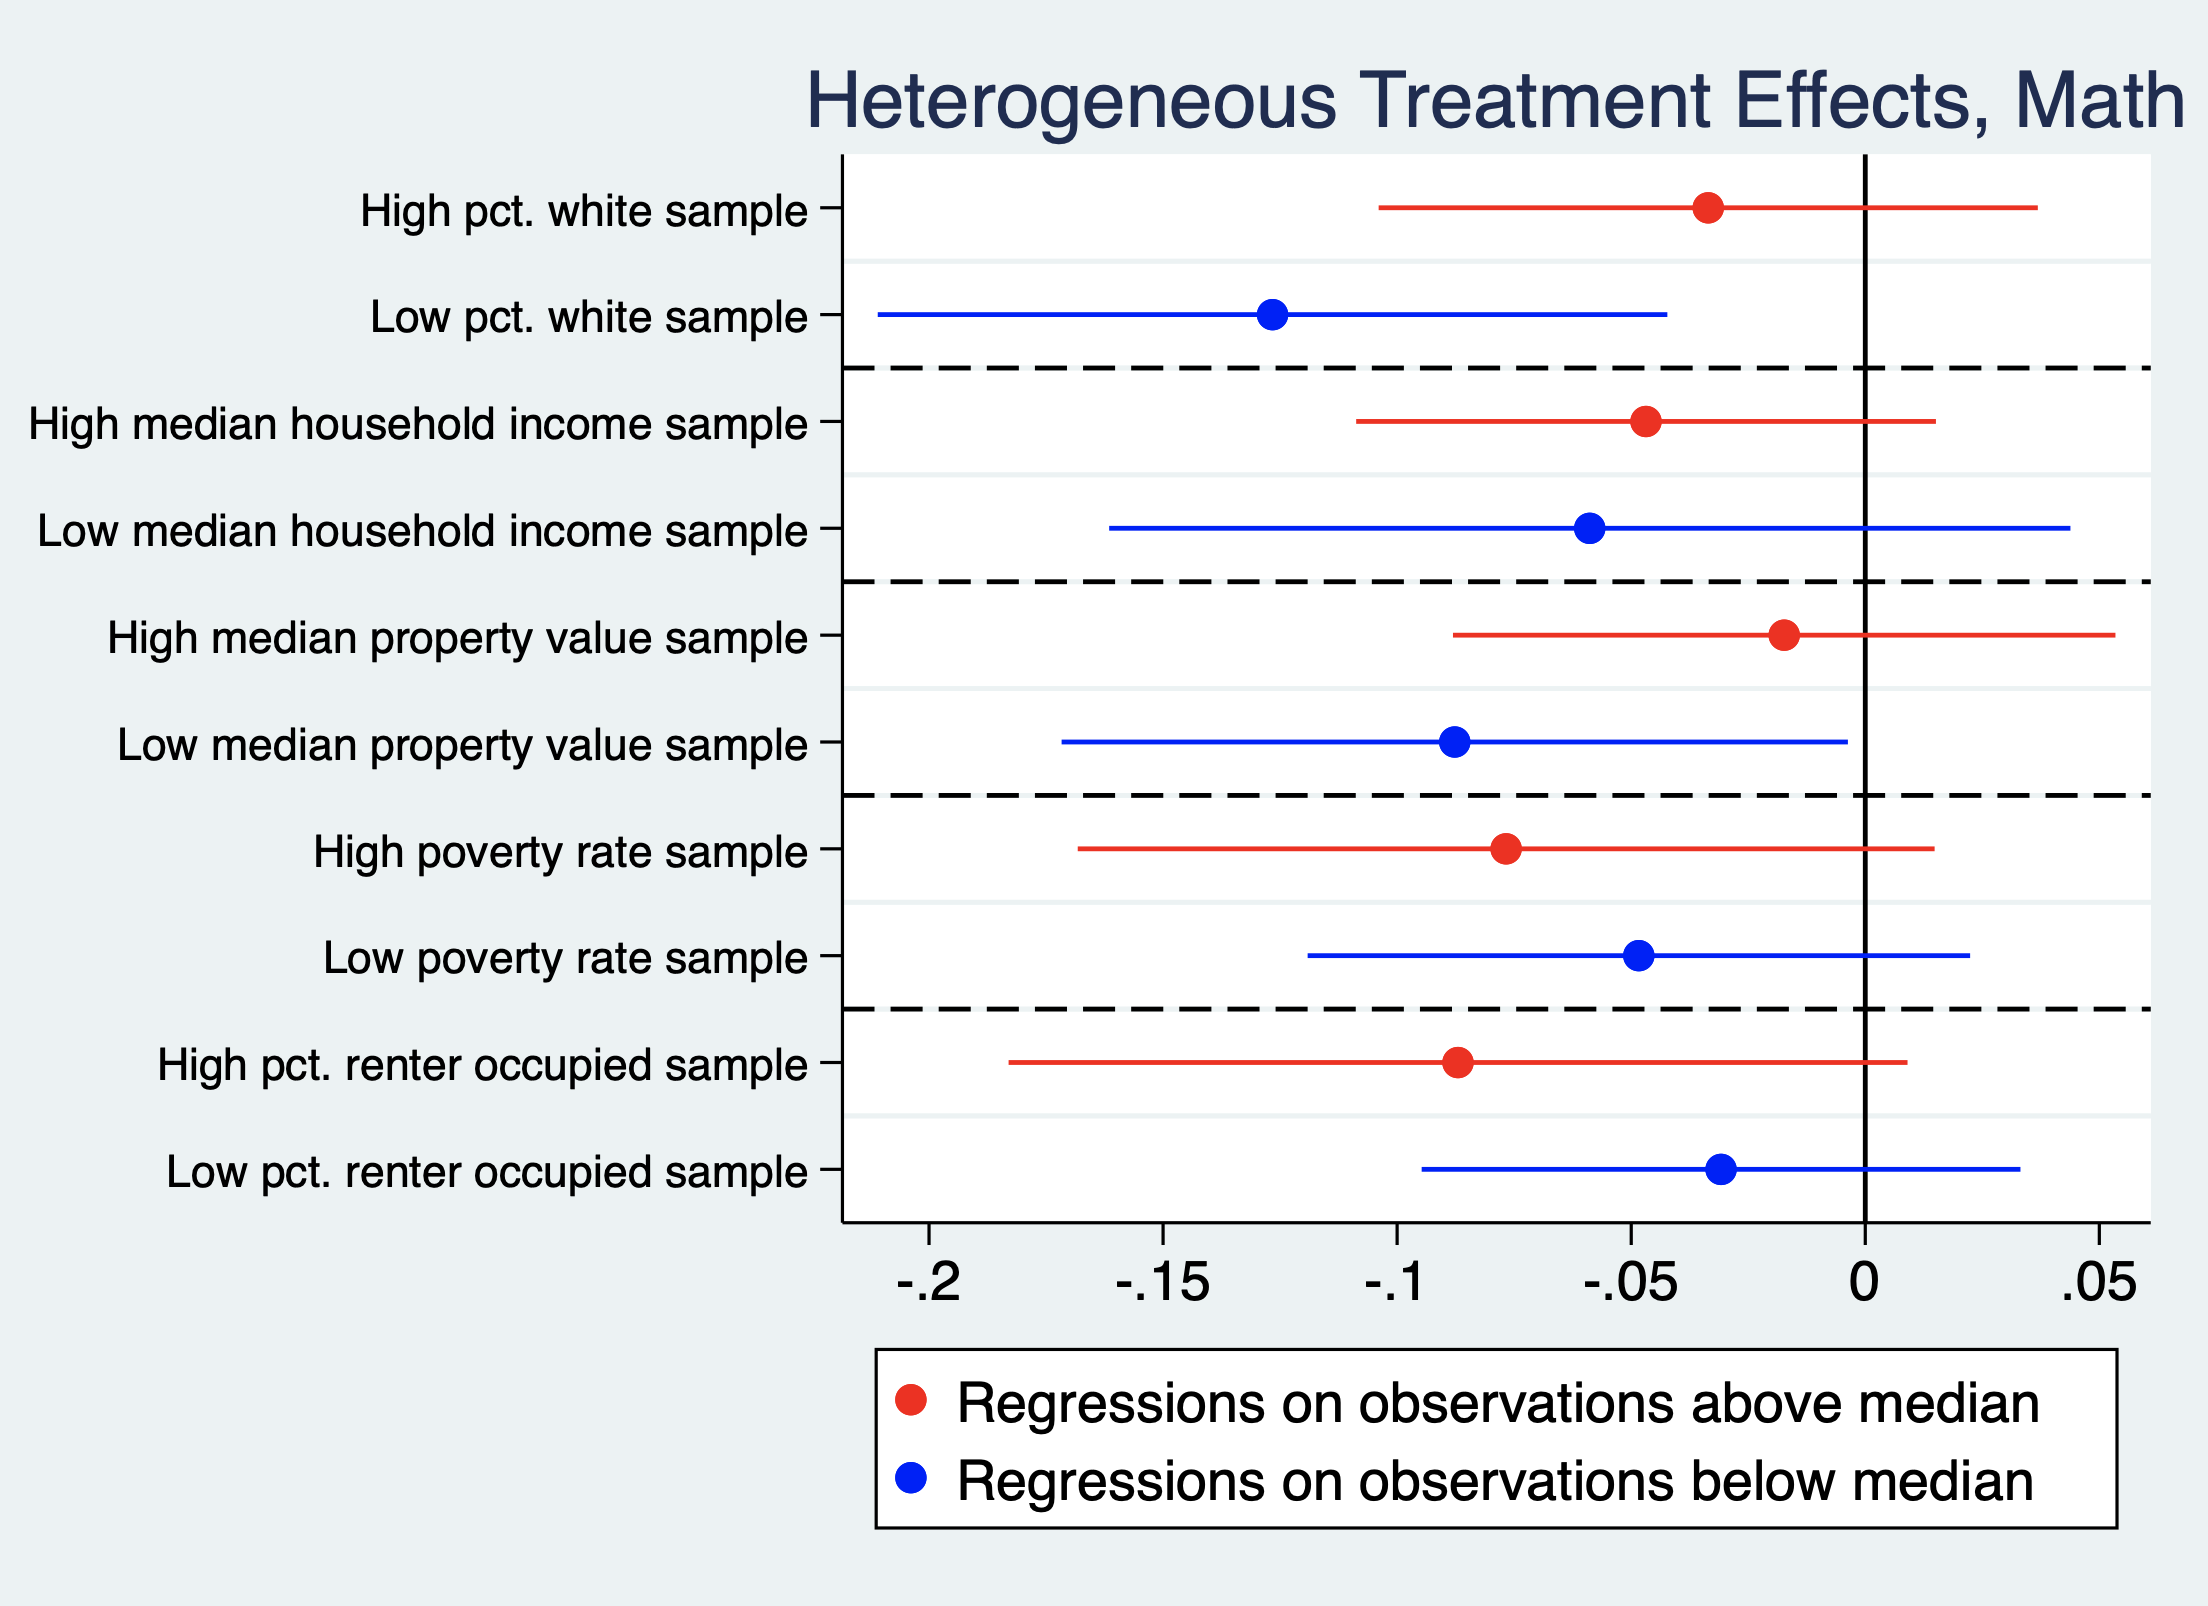
\includegraphics[scale=0.5]{output/graphs/math_heterogeneous_effects.png}
    \caption{}
    \label{fig:my_label}
\end{figure}
\end{landscape}

\begin{landscape}

\begin{figure}
    \centering
    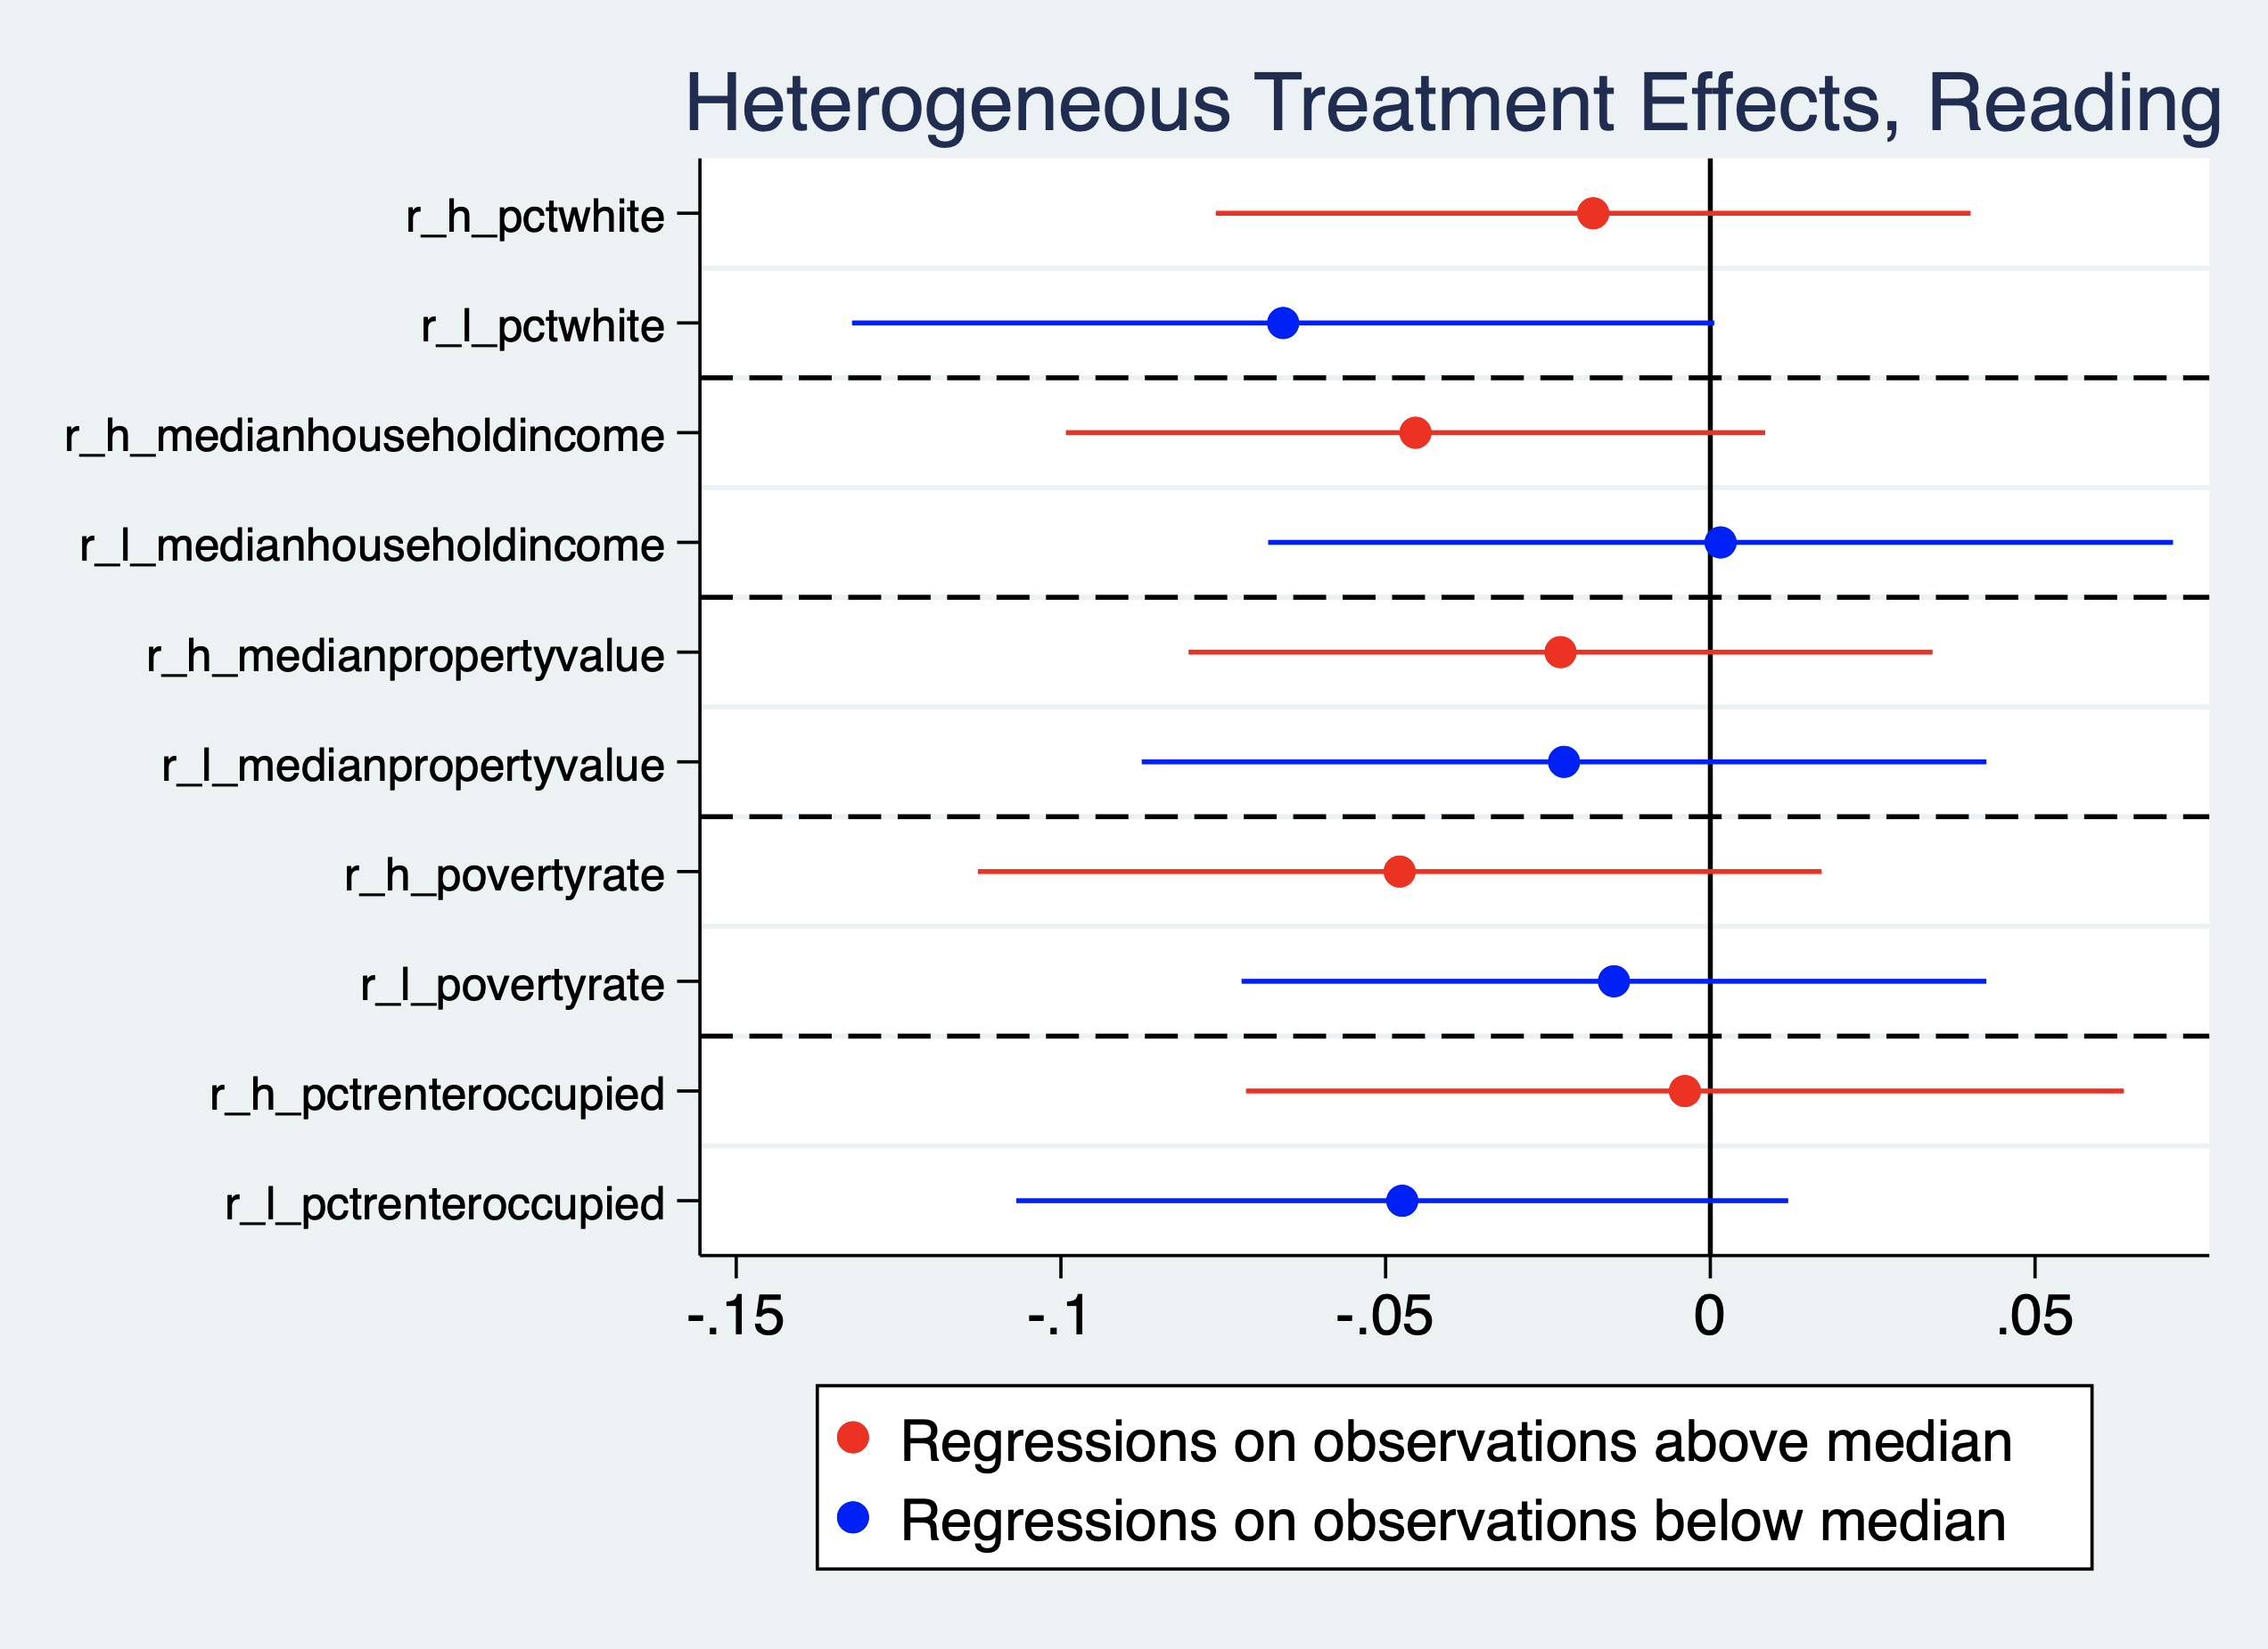
\includegraphics[scale=0.5]{output/graphs/read_heterogeneous_effects.png}
    \caption{}
    \label{fig:my_label}
\end{figure}
\end{landscape}
\section*{Appendix A. Placeholder} \label{sec:appendixa}

\addcontentsline{toc}{section}{Appendix A}



\end{document}